\documentclass[11pt,letterpaper]{article}

\usepackage{fontspec}
\usepackage[spanish,es-tabla,es-nodecimaldot]{babel}
\usepackage[margin=2.5cm]{geometry}
\usepackage{amsmath}
\usepackage{graphicx}
\usepackage{booktabs}
\usepackage{tabularx}
\usepackage{array}
\usepackage{multirow}
\usepackage{enumitem}
\usepackage{xcolor}
\usepackage[labelfont=bf,font=small]{caption}
\usepackage{subcaption}
\usepackage{float}
\usepackage{tikz}
\usetikzlibrary{arrows.meta,positioning,shapes.geometric,calc,automata,babel}
\usepackage[hidelinks]{hyperref}

\setlength{\parskip}{6pt}
\setlength{\emergencystretch}{3em}
\setlength{\parindent}{0pt}
\setlist{itemsep=2pt,topsep=4pt}
\graphicspath{{img/}}

\newcommand{\pend}[1]{\textcolor{red}{\textbf{[PENDIENTE: #1]}}}
\newcommand{\code}[1]{\texttt{#1}}

\begin{document}

% =============================================================== PORTADA
\begin{titlepage}
\centering
{\large\bfseries Universidad de las Américas Puebla\par}
\vspace{4pt}
Escuela de Ingeniería\par
\vspace{2pt}
Departamento de Computación, Electrónica y Mecatrónica\par
\vspace{2.2cm}
{\bfseries Sistemas Embebidos\par}
\vspace{4pt}
Proyecto Final\par
\vspace{1.4cm}
\rule{\linewidth}{0.6pt}\par
\vspace{10pt}
{\LARGE\bfseries Dispensador hospitalario de medicamento líquido con autenticación Face ID y control en FPGA DE10-Lite\par}
\vspace{10pt}
\rule{\linewidth}{0.6pt}\par
\vspace{1.6cm}
\begin{tabular}{ll}
\textbf{Estudiante} & \textbf{ID} \\
\midrule
Victor Hugo De La Calleja Mojica & 181626 \\
Rodrigo Daniel Carretero Santamaría & 180293 \\
\end{tabular}
\vfill
\begin{tabular}{rl}
\textbf{Curso:} & Sistemas Embebidos \\
\textbf{Profesor:} & Dr. Gerardo Ulises Díaz Arango \\
\textbf{Fecha:} & 27 de noviembre de 2026 \\
\textbf{Periodo:} & Otoño 2026 \\
\textbf{Repositorio:} & \url{https://github.com/CrazzyCoderHacker/dispensador-fpga-faceid} \\
\end{tabular}
\end{titlepage}

% =============================================================== RESUMEN
\section*{Resumen}
En un hospital, una bomba de infusión con llaves accesibles permite que un paciente o un familiar cambie el flujo o se administre dosis extra de un medicamento, por ejemplo un analgésico. Para evitarlo construimos un dispensador de medicamento líquido sobre una FPGA Terasic DE10-Lite (Intel MAX~10) en el que cada acción sensible pide Face ID en un iPhone. El iPhone verifica al usuario con una llave de acceso (\emph{passkey}) del estándar WebAuthn; un servidor en Python valida la firma y manda la orden a la FPGA por el mismo cable USB-Blaster con el que se programa, a través del bloque \emph{In-System Sources and Probes}. La FPGA decide todo lo demás: la sesión de enfermería con tiempo límite, los rangos de los parámetros, la identidad del paciente, la dosificación gota a gota en lazo cerrado, el límite de bolos tipo PCA y las alarmas. La bomba y la cámara de goteo no son físicas: las modelamos dentro de la misma FPGA, y las fallas se provocan con interruptores o desde la página. El diseño ocupa 2,595 elementos lógicos (5\,\% del dispositivo) y cumple la temporización a 50~MHz, con una frecuencia máxima de 72.81~MHz. Lo verificamos con 268 comprobaciones en simulación, 29 pruebas del servidor y nueve escenarios en la tarjeta. En la DE10-Lite, la FPGA detectó flujo libre en 0.7~s, ausencia de flujo en 5.6~s y apertura no autorizada del gabinete en 0.1~s, y rechazó parámetros fuera de rango, bolos dentro del tiempo de bloqueo y solicitudes hechas con el rostro de otra persona. Las pruebas en la tarjeta también sacaron a la luz dos errores del servidor que la simulación no había mostrado, y ambos quedaron corregidos. No usamos hardware aparte de la tarjeta, la laptop y el iPhone.

\textbf{Palabras clave:} FPGA, DE10-Lite, Verilog, Face ID, WebAuthn, passkeys, JTAG, bomba de infusión, analgesia controlada por el paciente.

{\setlength{\parskip}{0pt}\tableofcontents}
\newpage

% =============================================================== 1 INTRODUCCIÓN
\section{Introducción}
Una bomba de infusión entrega un medicamento líquido a una velocidad programada. La FDA reporta que estos equipos han tenido problemas de seguridad persistentes que pueden causar sobreinfusión, subinfusión o terapia omitida o retrasada, y que muchos se deben a deficiencias de diseño \cite{fda_pumps}. En equipos sencillos, o cuando el flujo se controla con una llave manual, el paciente o un acompañante puede abrir el paso o pedir más dosis de las indicadas. En la analgesia controlada por el paciente (PCA) esto se limita con un tiempo de bloqueo entre dosis y un máximo por hora, pero esas reglas solo sirven si nadie más puede pedir la dosis o cambiar el programa.

Para saber quién da cada orden usamos la biometría que ya trae el teléfono. Con WebAuthn \cite{webauthn}, el iPhone guarda una llave privada que solo usa después de reconocer el rostro con Face ID \cite{apple_passkeys,apple_biometric}. El servidor recibe una firma y la comprueba con la llave pública, sin conocer nunca la llave privada \cite{apple_passkeys}. Así cada orden queda ligada a una persona y no a quien tenga el teléfono en la mano.

Repartimos el trabajo en tres partes. El iPhone verifica al usuario con Face ID. El servidor, en la laptop, valida la respuesta de WebAuthn y convierte la orden en una palabra de 32 bits. La FPGA es el motor del dispensador: en ella corren la máquina de estados de la infusión, el control del goteo, la validación de cada orden, el límite de bolos y la detección de alarmas. Para no agregar módulos de comunicación, la laptop se comunica con la FPGA por el USB-Blaster de la tarjeta, el mismo cable con el que se programa. Como no compramos componentes, la bomba y la cámara de goteo están modeladas dentro de la FPGA. Por eso lo que probamos en la tarjeta es la lógica de control frente a condiciones físicas simuladas, no el comportamiento hidráulico de un equipo real.

Nos planteamos tres objetivos:
\begin{enumerate}
\item Implementar en la FPGA la función principal del dispensador: dosificación gota a gota en lazo cerrado, límite de bolos, detección de alarmas y validación de todas las órdenes.
\item Autenticar a la enfermera y al paciente con Face ID del iPhone y llevar sus órdenes a la FPGA sin agregar módulos de comunicación.
\item Verificar el diseño en simulación y en la tarjeta DE10-Lite, incluyendo los intentos de uso no autorizado y las fallas físicas del equipo.
\end{enumerate}

En la Sección~\ref{sec:metodologia} describimos el diseño y cómo lo probamos, en la Sección~\ref{sec:resultados} presentamos y discutimos los resultados, y en la Sección~\ref{sec:conclusiones} damos las conclusiones. El código Verilog, el proyecto de Quartus con el archivo de programación, el servidor, los bancos de prueba, las instrucciones de ejecución y las evidencias están en el repositorio \url{https://github.com/CrazzyCoderHacker/dispensador-fpga-faceid}.

% =============================================================== 2 METODOLOGÍA
\section{Metodología}\label{sec:metodologia}

\subsection{Fundamentos}
\textbf{Dosificación por gotas.} Un equipo de macrogoteo entrega un factor fijo de gotas por mililitro; en este proyecto $F = 20$~gotas/mL. Para una velocidad $Q$ en mL/h, el intervalo entre gotas es
\begin{equation}
T_{\text{gota}} = \frac{3\,600\,000}{Q \cdot F}\ \text{ms},
\label{eq:intervalo}
\end{equation}
de modo que 360~mL/h corresponden a una gota cada 500~ms y 999~mL/h a una cada 180~ms. El volumen total a infundir (VTBI) define el número de gotas objetivo $N = V_{\text{TBI}} \cdot F$.

\textbf{Control en lazo cerrado.} Un programador interno incrementa un contador de gotas programadas $n_s$ cada $T_{\text{gota}}$. La bomba se enciende solo mientras las gotas entregadas $n_d$ son menores que las programadas:
\begin{equation}
\text{bomba} = (\text{estado} = \text{RUN}) \land (n_d < n_s).
\label{eq:bomba}
\end{equation}
Así la bomba entrega exactamente las gotas programadas aunque su caudal real varíe. Las mismas cuentas permiten supervisar el equipo: si la bomba está encendida y no caen gotas hay una obstrucción, y si caen más gotas de las programadas alguien abrió el paso del líquido.

\textbf{Passkeys y Face ID.} En el registro, el iPhone genera un par de llaves para el dominio de la página y entrega solo la llave pública al servidor. La llave privada se guarda en el llavero de iCloud y no se comparte con el servidor \cite{apple_passkeys}. En cada autenticación el servidor envía un reto aleatorio, el iPhone pide Face ID y firma el reto con la llave privada \cite{webauthn,apple_biometric}. El servidor exige la bandera de verificación de usuario (UV), con lo que la firma solo es válida si Face ID tuvo éxito. WebAuthn solo funciona en un contexto seguro (HTTPS) con nombre de dominio, lo que define la forma de conectar el iPhone (Sección~\ref{sec:servidor}).

\subsection{Arquitectura del sistema}
La Figura~\ref{fig:arquitectura} muestra los tres elementos del sistema. El iPhone es la interfaz de enfermería y del paciente; la laptop verifica las firmas de Face ID y transporta órdenes; la FPGA aplica todas las reglas y controla la infusión. La laptop se conecta a la tarjeta con un solo cable USB, el mismo del programador USB-Blaster integrado en la DE10-Lite \cite{de10lite}.

\begin{figure}[H]
\centering
\begin{tikzpicture}[
  box/.style={draw, rounded corners=3pt, align=center, minimum height=1.7cm, text width=3.3cm, font=\small},
  arr/.style={-{Stealth[length=2.2mm]}, thick}]
\node[box, fill=blue!6] (phone) {\textbf{iPhone (Safari)}\\Face ID\\Llave privada\\(passkey)};
\node[box, fill=gray!10, right=2.3cm of phone] (laptop) {\textbf{Laptop}\\Servidor Flask\\Verifica la firma\\\code{quartus\_stp}};
\node[box, fill=orange!10, right=2.3cm of laptop] (fpga) {\textbf{DE10-Lite (MAX 10)}\\Sesión, rangos,\\bolos, lazo de\\goteo, alarmas};
\draw[arr] ([yshift=3mm]phone.east) -- node[above, font=\scriptsize]{firma, orden} ([yshift=3mm]laptop.west);
\draw[arr] ([yshift=-3mm]laptop.west) -- node[below, font=\scriptsize]{estado} ([yshift=-3mm]phone.east);
\draw[arr] ([yshift=3mm]laptop.east) -- node[above, font=\scriptsize]{orden 32 bits} ([yshift=3mm]fpga.west);
\draw[arr] ([yshift=-3mm]fpga.west) -- node[below, font=\scriptsize]{estado 224 bits} ([yshift=-3mm]laptop.east);
\node[font=\scriptsize, below=0.5cm of $(phone.south)!0.5!(laptop.south)$] {HTTPS (túnel)};
\node[font=\scriptsize, below=0.5cm of $(laptop.south)!0.5!(fpga.south)$] {USB-Blaster (JTAG)};
\end{tikzpicture}
\caption{Arquitectura del dispensador. La laptop solo verifica la identidad y transporta órdenes; la FPGA decide.}
\label{fig:arquitectura}
\end{figure}

Como no se adquirió ningún componente, la bomba peristáltica y la cámara de goteo se modelan dentro de la FPGA. Las fallas físicas (llave abierta, tubo tapado y gabinete abierto) se simulan con interruptores de la tarjeta o desde un panel de demostración de la página. En ambos casos la FPGA solo recibe la condición física y debe detectarla por sí misma, igual que con un sensor real.

\subsection{Diseño en la FPGA}
El diseño se escribió en Verilog-2001 \cite{verilog} con 12 módulos y 1,294 líneas, sobre el reloj de 50~MHz de la tarjeta. Sus componentes principales son:
\begin{itemize}
\item \textbf{cmd\_ctrl:} recibe las órdenes por JTAG y aplica roles, sesión de enfermería de 120~s que se renueva con cada orden, rangos de los parámetros e identidad del paciente.
\item \textbf{infusion\_ctrl:} máquina de estados de la infusión, programador de gotas, lazo cerrado de la Ecuación~\eqref{eq:bomba} y supervisión de alarmas.
\item \textbf{divu:} divisor secuencial de 32 bits que calcula la Ecuación~\eqref{eq:intervalo} sin multiplicadores ni divisores combinacionales.
\item \textbf{bolus\_limiter:} limitador tipo PCA con tiempo de bloqueo y ventana deslizante de 60~minutos con las marcas de tiempo de los últimos 8 bolos.
\item \textbf{drip\_sim:} modelo de bomba y cámara de goteo; produce una gota cada 150~ms con la bomba encendida, una cada 120~ms con la llave abierta y ninguna con el tubo tapado.
\item \textbf{jtag\_link:} instancia el bloque \code{altsource\_probe} con una fuente de 32 bits y una sonda de 224 bits \cite{issp}.
\item \textbf{Soporte:} generador de bases de tiempo, sincronizadores con antirrebote, PWM, zumbador, conversión binario-BCD y caracteres de siete segmentos \cite{chu}.
\end{itemize}

La Figura~\ref{fig:fsm} muestra la máquina de estados de la infusión. Toda alarma apaga la bomba, y solo una enfermera con sesión puede atenderla; la infusión queda entonces en pausa y debe reiniciarse de forma explícita.

\begin{figure}[H]
\centering
\begin{tikzpicture}[->, >={Stealth[length=2.2mm]}, node distance=3.2cm, thick,
  every state/.style={minimum size=1.35cm, font=\small, fill=gray!8},
  lbl/.style={font=\scriptsize, align=center}]
\node[state, initial, initial text={}] (idle) {IDLE};
\node[state, right=of idle] (run) {RUN};
\node[state, right=of run] (done) {DONE};
\node[state, below=2.2cm of run] (pause) {PAUSE};
\node[state, fill=red!12, below=2.2cm of done] (alarm) {ALARM};
\draw (idle) -- node[above, lbl]{START\\(sesión)} (run);
\draw (run) -- node[above, lbl]{$n_d \ge N$} (done);
\draw (run) to[bend right=20] node[left, lbl]{pausa} (pause);
\draw (pause) to[bend right=20] node[right, lbl]{START\\(sesión)} (run);
\draw (run) -- node[above right, lbl]{falla} (alarm);
\draw (alarm) -- node[below, lbl]{atender (sesión)} (pause);
\draw (pause) -| node[pos=0.25, below, lbl]{bolsa nueva} (idle);
\end{tikzpicture}
\caption{Máquina de estados de la infusión. Desde IDLE y PAUSE también se entra a ALARM si caen gotas sin infusión o se abre el gabinete sin sesión.}
\label{fig:fsm}
\end{figure}

Las alarmas y sus condiciones de disparo se resumen en la Tabla~\ref{tab:alarmas}.

\begin{table}[H]
\centering
\caption{Alarmas detectadas por la FPGA.}
\label{tab:alarmas}
\begin{tabularx}{\linewidth}{lXl}
\toprule
\textbf{Alarma} & \textbf{Condición en la FPGA} & \textbf{Pantalla} \\
\midrule
Sin flujo & Bomba encendida 5~s sin detectar gotas (bolsa vacía o tubo tapado) & \code{AL noFL} \\
Flujo libre & $n_d > n_s + 3$ durante la infusión, o 3 gotas con la infusión detenida & \code{AL FrEE} \\
Manipulación & Gabinete abierto sin sesión de enfermería & \code{AL tAPA} \\
\bottomrule
\end{tabularx}
\end{table}

Los controles de la tarjeta se asignaron de la siguiente forma. KEY0 reinicia el sistema y KEY1 pausa la infusión localmente. SW9 activa el modo demostración, en el que un minuto clínico dura un segundo. SW7, SW6 y SW5 simulan la llave abierta, el tubo tapado y el gabinete abierto, y SW1--SW0 eligen el valor mostrado. Los displays HEX5--HEX4 muestran el estado (\code{id}, \code{ru}, \code{PA}, \code{AL}, \code{dn}) y HEX3--HEX0 el valor o el nombre de la alarma. Los LEDs indican sesión (LEDR0), bomba (LEDR1), gota (LEDR2), bolo concedido (LEDR3), orden rechazada (LEDR4), gabinete abierto (LEDR5) y alarma (LEDR9).

\subsection{Protocolo de comunicación por JTAG}\label{sec:jtag}
El bloque \emph{In-System Sources and Probes} de Quartus agrega al diseño registros que la laptop lee y escribe por la cadena JTAG \cite{issp,jtag}. El servidor ejecuta \code{quartus\_stp} en modo interactivo y usa los comandos Tcl \code{write\_source\_data} y \code{read\_probe\_data} del paquete \code{::quartus::insystem\_source\_probe}, descritos en la interfaz Tcl del mismo bloque \cite{issp}. No se usó UART, Wi-Fi ni ningún otro módulo.

Cada orden es una palabra de 32 bits con el formato \code{[31:24]} secuencia, \code{[23:20]} operación y \code{[19:0]} argumento. La FPGA sincroniza la palabra con tres registros, la ejecuta cuando la secuencia cambia y permanece estable en dos muestras, y publica en la sonda el número de secuencia atendido y un código de resultado. La Tabla~\ref{tab:ordenes} lista las operaciones. La sonda de 224 bits contiene además el estado, la alarma, la sesión, los parámetros, el volumen entregado, el bloqueo restante y un historial de los cuatro últimos eventos con contador, con el que el servidor reconstruye la bitácora.

\begin{table}[H]
\centering
\caption{Órdenes que acepta la FPGA y reglas que aplica a cada una.}
\label{tab:ordenes}
\begin{tabularx}{\linewidth}{clX}
\toprule
\textbf{Op} & \textbf{Orden} & \textbf{Regla aplicada en la FPGA} \\
\midrule
1 & LOGIN(id) & Solo IDs 1--49 (enfermería) abren sesión de 120~s \\
2 & LOGOUT & Cierra la sesión activa \\
3 & SET(sel, valor) & Requiere sesión; velocidad 1--999~mL/h, volumen 1--999~mL, bolo 0--50~mL, bloqueo 0--240~min, 0--8 bolos/h, paciente 0 o 50--99 \\
4 & START & Requiere sesión y un programa válido \\
5 & PAUSA / ATENDER & Pausar siempre se permite; atender alarma o bolsa nueva requiere sesión \\
6 & BOLO(id) & El id debe ser el del paciente asignado; después decide el limitador \\
7 & SIM(fallas) & Solo demostración: simula condiciones físicas, no otorga permisos \\
\bottomrule
\end{tabularx}
\end{table}

Los códigos de resultado son 0 (aceptada), 1 (el ID no es de enfermería), 2 (sin sesión), 3 (fuera de rango), 4 (rostro de otro paciente) y 5 (orden desconocida).

Elegimos este enlace porque la DE10-Lite ya trae el USB-Blaster integrado \cite{de10lite}: con un solo cable programamos la FPGA y mandamos las órdenes, sin comprar un módulo UART o Wi-Fi. A cambio, el sistema depende de que la laptop siga conectada por USB y tenga Quartus instalado, porque todas las órdenes pasan por \code{quartus\_stp}.

Cada orden sigue el mismo intercambio. Primero, el servidor abre la conexión una sola vez al arrancar: busca el USB-Blaster con \code{get\_hardware\_names}, el MAX~10 con \code{get\_device\_names} e inicia el acceso con \code{start\_insystem\_source\_probe}. Después, para mandar una orden, incrementa el número de secuencia, arma la palabra de 32 bits y la escribe con \code{write\_source\_data}. La FPGA solo la ejecuta cuando la secuencia cambia y la palabra se mantiene igual en dos muestras seguidas, así que una escritura a medias nunca se ejecuta y una misma orden nunca se repite. Al terminar, la FPGA copia la secuencia atendida y el código de resultado en la sonda. Por último, el servidor lee la sonda con \code{read\_probe\_data} hasta encontrar su número de secuencia; si no aparece en 2~s, reporta que la FPGA no respondió. Una lectura completa de la sonda tarda unos 7~ms en la tarjeta. La Tabla~\ref{tab:sonda} resume el contenido de la sonda.

\begin{table}[H]
\centering
\caption{Mapa del registro de estado (sonda de 224 bits).}
\label{tab:sonda}
\begin{tabular}{ll|ll}
\toprule
\textbf{Bits} & \textbf{Campo} & \textbf{Bits} & \textbf{Campo} \\
\midrule
\code{[7:0]} & Secuencia atendida & \code{[83:76]} & ID del paciente asignado \\
\code{[11:8]} & Código de resultado & \code{[91:84]} & Bloqueo restante (min) \\
\code{[14:12]} & Estado de la infusión & \code{[95:92]} & Bolos en la última hora \\
\code{[16:15]} & Alarma & \code{[103:96]} & Sesión restante (s) \\
\code{[17]} & Sesión activa & \code{[111:104]} & Contador de eventos \\
\code{[25:18]} & ID de la enfermera & \code{[207:112]} & Últimos 4 eventos (24 bits c/u) \\
\code{[35:26]} & mL entregados & \code{[208]} & Bomba encendida \\
\code{[45:36]} & Velocidad (mL/h) & \code{[209]} & Gabinete abierto \\
\code{[55:46]} & Volumen (mL) & \code{[212:210]} & Fallas presentes \\
\code{[75:56]} & Bolo, bloqueo y máx./hora & \code{[215:213]} & Fallas pedidas por el panel \\
\bottomrule
\end{tabular}
\end{table}

\subsection{Servidor y Face ID}\label{sec:servidor}
El servidor se escribió en Python con Flask \cite{flask} y la biblioteca \code{py\_webauthn} \cite{pywebauthn}. Sus funciones son:
\begin{itemize}
\item \textbf{Registro:} protegido con un PIN de administrador; asocia cada passkey con un rol y un ID (enfermería 1--49, pacientes 50--99) y exige autenticador de plataforma, credencial residente y verificación de usuario.
\item \textbf{Autenticación:} genera un reto por solicitud y verifica origen, dominio, firma, contador y la bandera UV antes de mandar cualquier orden a la FPGA.
\item \textbf{Bolo:} solo una passkey de paciente puede solicitarlo; la FPGA comprueba que sea el paciente asignado y el limitador decide si se concede.
\item \textbf{Página:} interfaz en español para enfermería, paciente, simulador de fallas y bitácora, que lee el estado de la FPGA cada 700~ms.
\end{itemize}

Para obtener HTTPS con nombre de dominio sin comprar ni configurar un servidor, la página se publicó con un túnel rápido de Cloudflare \cite{cloudflare}, que asigna una dirección \code{https://*.trycloudflare.com} temporal. El iPhone abre esa dirección en Safari con datos móviles o cualquier red Wi-Fi.

\subsection{Página segura (HTTPS)}\label{sec:https}
WebAuthn solo funciona en un contexto seguro, es decir, en una página servida por HTTPS con nombre de dominio \cite{webauthn}. Con la dirección IP de la laptop, Safari no permite crear ni usar passkeys. Para resolverlo usamos el túnel rápido de Cloudflare \cite{cloudflare}. El programa \code{cloudflared} abre desde la laptop una conexión de salida hacia Cloudflare, y Cloudflare publica la página en una dirección \code{https://*.trycloudflare.com} con su propio certificado. De esta forma, la conexión entre el iPhone y Cloudflare va cifrada con TLS, la conexión entre Cloudflare y la laptop viaja dentro del túnel, y no tuvimos que abrir puertos en la red ni comprar un dominio o un certificado.

El servidor sigue escuchando solo en el puerto 5000 de la laptop. Para validar cada firma toma el dominio y el protocolo con los que el iPhone abrió la página (cabeceras \code{X-Forwarded-Host} y \code{X-Forwarded-Proto}) y los usa como identificador del sitio (RP ID) y como origen esperado. Así, una firma hecha para otro dominio no se acepta. La desventaja es que la dirección del túnel cambia cada vez que se reinicia \code{cloudflared}, y como cada passkey queda ligada a esa dirección, hay que registrar de nuevo los rostros.

\subsection{Medidas de seguridad y retroalimentación de la FPGA}\label{sec:seguridad}
Diseñamos la seguridad en capas, de modo que una orden indebida tenga que pasar varias revisiones antes de afectar la infusión. La Tabla~\ref{tab:seguridad} resume cada medida y dónde se aplica.

\begin{table}[H]
\centering
\caption{Medidas de seguridad del dispensador.}
\label{tab:seguridad}
\begin{tabularx}{\linewidth}{lX}
\toprule
\textbf{Medida} & \textbf{Qué evita} \\
\midrule
\multicolumn{2}{l}{\textit{iPhone y servidor}} \\
Passkey con Face ID obligatorio (UV) & Que alguien firme sin que el iPhone reconozca su rostro \\
Autenticador de la plataforma y credencial residente & Que se use una llave externa en lugar del Face ID del teléfono \\
Reto aleatorio de un solo uso & Que se reenvíe una firma vieja capturada antes \\
Verificación de origen, dominio y contador de firmas & Firmas hechas para otra página o credenciales clonadas \\
PIN de administrador para registrar rostros & Que cualquiera registre su cara como enfermera \\
Roles en el servidor & Que un paciente programe la bomba o que una enfermera pida el bolo del paciente \\
\midrule
\multicolumn{2}{l}{\textit{FPGA}} \\
Sesión de enfermería de 120~s & Que una sesión olvidada quede abierta \\
IDs por rol (1--49 y 50--99) & Que un ID de paciente abra sesión de enfermería \\
Rangos de cada parámetro & Velocidades o volúmenes peligrosos, aunque el servidor falle \\
Paciente asignado y limitador de bolos & Bolos de otra persona, dentro del bloqueo o sobre el máximo por hora \\
Pausa siempre permitida & Que una falla de autenticación impida detener la bomba \\
\bottomrule
\end{tabularx}
\end{table}

La FPGA no confía en el servidor: vuelve a revisar sesión, roles, rangos y paciente asignado en cada orden. Por eso, si la laptop llegara a enviar una orden indebida, la FPGA la rechazaría aunque la firma de Face ID hubiera sido válida.

La FPGA también le regresa al sistema el resultado de todo lo que hace, por tres caminos. El primero es el acuse de cada orden: la secuencia atendida y un código de resultado (aceptada, ID que no es de enfermería, sin sesión, fuera de rango, rostro de otro paciente u orden desconocida), con el que el servidor arma el mensaje que ve el usuario en el iPhone. El segundo es la bitácora: la FPGA guarda los últimos cuatro eventos con un contador, y el servidor detecta los eventos nuevos para mostrarlos en la página, como sesiones, parámetros cambiados, bolos concedidos o negados, alarmas y órdenes rechazadas. En el caso del bolo, el servidor espera este evento antes de responder, porque el acuse solo indica que la orden llegó y no si el limitador la concedió. El tercero es la propia tarjeta: los displays muestran el estado y la alarma, y los LEDs indican sesión, bomba, gota, bolo concedido, orden rechazada, gabinete abierto y alarma, de modo que el estado se puede revisar aunque la laptop esté desconectada.

\subsection{Entorno de pruebas}
La síntesis, el ajuste y el análisis de tiempos se realizaron con Quartus Prime Lite Edition 25.1 para el dispositivo 10M50DAF484C7G. La simulación se realizó con Icarus Verilog \cite{iverilog}, sustituyendo el bloque JTAG por un modelo cuyo registro de fuente escribe el banco de pruebas. De esta forma, la prueba de sistema actúa como la laptop: manda órdenes y lee la sonda con el mismo mapa de bits que usa el servidor. El servidor se probó con un autenticador de software P-256 que genera respuestas WebAuthn válidas y alteradas.

Las pruebas en la tarjeta siguieron siempre los mismos pasos: reiniciar con KEY0, abrir sesión de enfermería, cargar el programa con el paciente 55, iniciar la infusión y provocar cada caso. Las fotografías se tomaron con la orden enviada directamente por el enlace JTAG, y la autenticación con Face ID se probó por separado desde el iPhone.

% =============================================================== 3 RESULTADOS
\section{Resultados y discusión}\label{sec:resultados}

\subsection{Síntesis en Quartus}
El proyecto compiló sin errores. La Tabla~\ref{tab:recursos} resume los recursos. El diseño usa el 5\,\% de los elementos lógicos y ningún bloque de memoria, multiplicador ni PLL, porque el intervalo de goteo se calcula con un divisor secuencial. El análisis de tiempos en el modelo lento a 85\,°C dio una frecuencia máxima de 72.81~MHz para el reloj de 50~MHz, con holgura positiva de 5.56~ns, y de 98.48~MHz para el reloj JTAG.

\begin{table}[H]
\centering
\caption{Recursos del diseño en el MAX 10 10M50DAF484C7G.}
\label{tab:recursos}
\begin{tabular}{lrr}
\toprule
\textbf{Recurso} & \textbf{Usado} & \textbf{Disponible} \\
\midrule
Elementos lógicos & 2,595 (5\,\%) & 49,760 \\
Funciones combinacionales & 2,269 (5\,\%) & 49,760 \\
Registros & 1,402 (3\,\%) & 49,760 \\
Pines & 107 (30\,\%) & 360 \\
Bits de memoria, multiplicadores, PLL & 0 & --- \\
Frecuencia máxima (reloj de 50~MHz) & 72.81~MHz & --- \\
\bottomrule
\end{tabular}
\end{table}

El 30\,\% de pines corresponde a los displays, LEDs, interruptores y el conector GPIO, que se dejó asignado para conectar una bomba y un sensor reales en una versión futura.

\subsection{Verificación por simulación}
La Tabla~\ref{tab:simulacion} resume las pruebas. Todas pasaron. La prueba de sistema recorre la secuencia completa de uso: órdenes sin sesión, sesión con un ID de paciente, programación con valores fuera de rango, infusión, bolos del paciente correcto y de otra persona, las tres alarmas por interruptor y por orden de simulación, pausa local y fin de la infusión. A 360~mL/h, el modelo entregó entre 5 y 7 gotas en 3~s, de acuerdo con la Ecuación~\eqref{eq:intervalo}.

\begin{table}[H]
\centering
\caption{Pruebas automáticas y resultados.}
\label{tab:simulacion}
\begin{tabularx}{\linewidth}{lXr}
\toprule
\textbf{Prueba} & \textbf{Qué verifica} & \textbf{Resultado} \\
\midrule
tb\_divu & Divisor secuencial contra el cociente exacto & 205/205 \\
tb\_bolus\_limiter & Bloqueo, máximo por hora y ventana de 60~min & 10/10 \\
tb\_infusion\_ctrl & Lazo cerrado, alarmas, pausa y fin & 20/20 \\
tb\_system & Sistema completo con órdenes por JTAG & 33/33 \\
test\_server & WebAuthn, roles, firmas alteradas, UV, bolos y simulación & 29/29 \\
\bottomrule
\end{tabularx}
\end{table}

La prueba del servidor confirmó que una firma alterada y una respuesta sin verificación de usuario se rechazan, que una enfermera no puede pedir el bolo del paciente y que, sin sesión, el navegador ya no puede mandar órdenes.

\subsection{Operación en la tarjeta}
La Figura~\ref{fig:inicio} muestra la tarjeta en reposo y después de que la enfermera abrió sesión con Face ID y cargó el programa. El enlace JTAG leyó el estado completo en aproximadamente 7~ms por lectura, suficiente para actualizar la página cada 700~ms.

\begin{figure}[H]
\centering
\begin{subfigure}{0.32\linewidth}\centering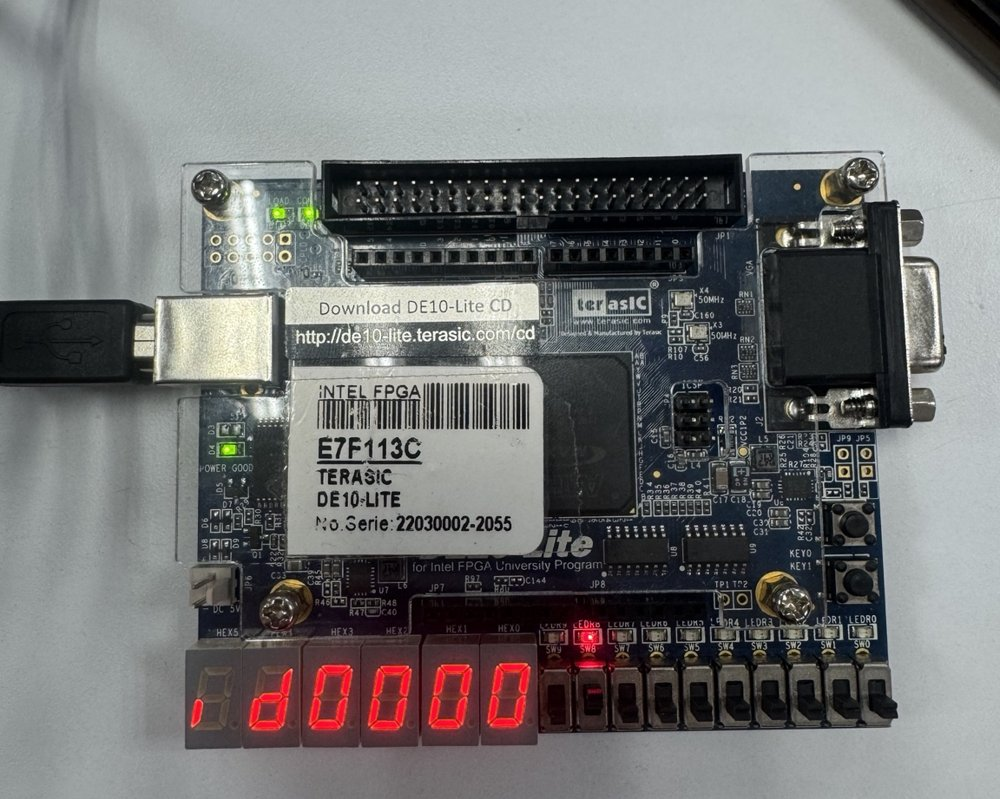
\includegraphics[width=\linewidth]{fpga_inactivo.jpg}\caption{Reposo (\code{id})}\end{subfigure}\hfill
\begin{subfigure}{0.32\linewidth}\centering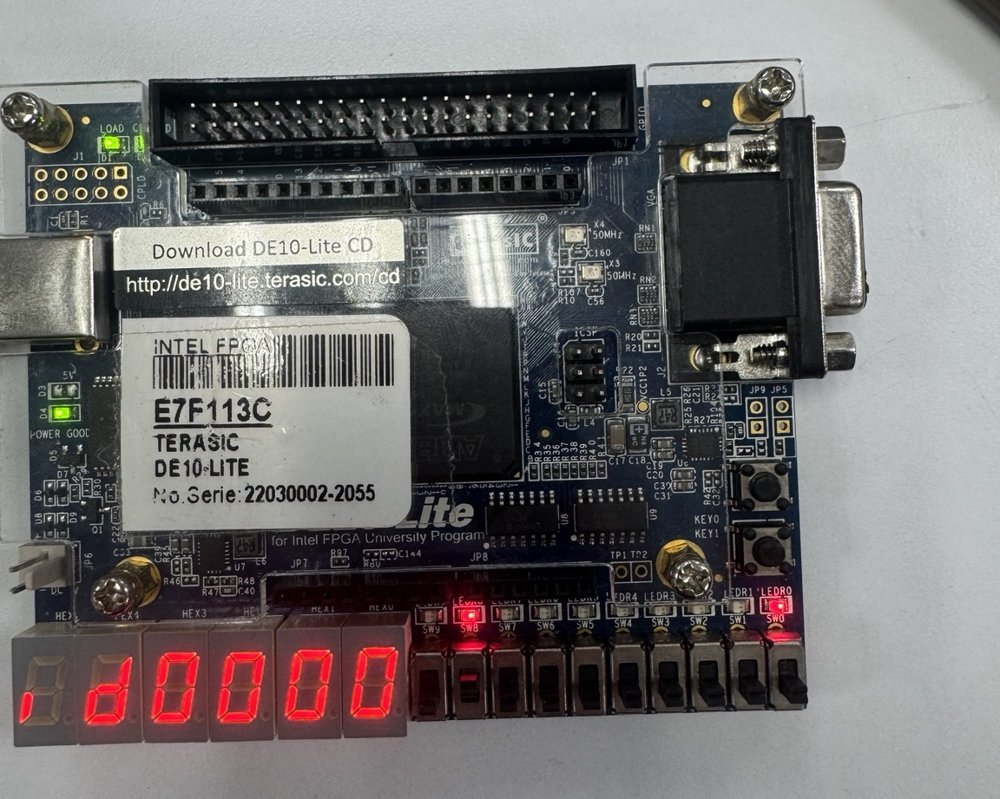
\includegraphics[width=\linewidth]{fpga_sesion.jpg}\caption{Sesión abierta (LEDR0)}\end{subfigure}\hfill
\begin{subfigure}{0.32\linewidth}\centering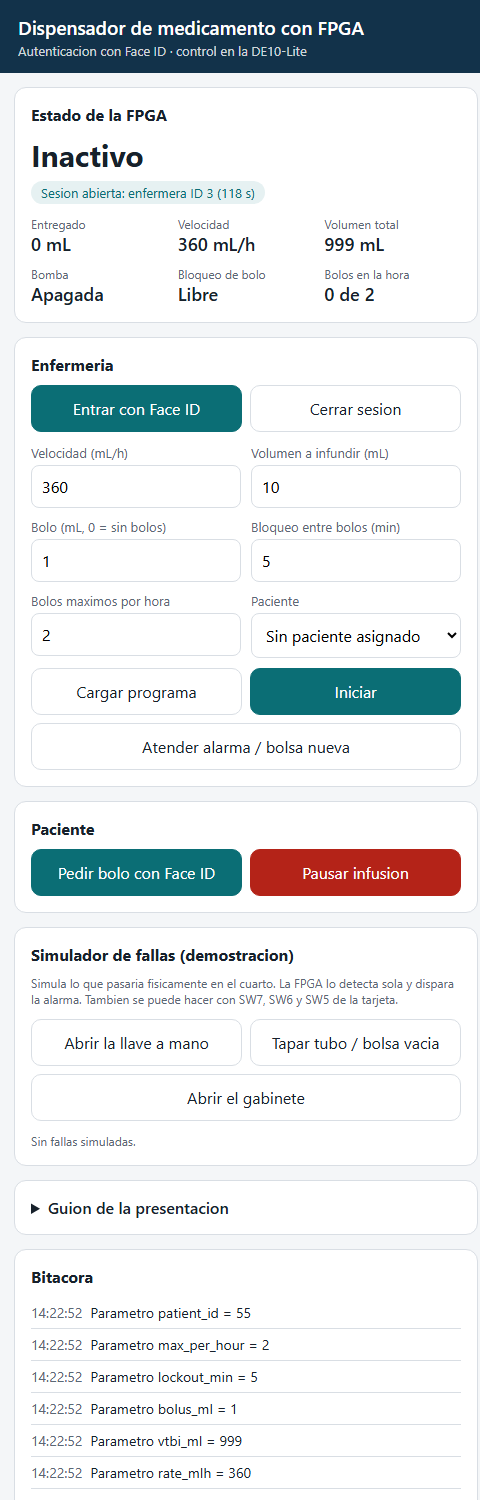
\includegraphics[width=\linewidth,trim=0 1170 0 0,clip]{web_programa.png}\caption{Programa cargado}\end{subfigure}
\caption{Inicio de la operación: equipo en reposo, sesión de enfermería y programa en la página.}
\label{fig:inicio}
\end{figure}

La autenticación con Face ID funcionó desde un iPhone a través del túnel HTTPS: el registro guardó la passkey en el llavero de iCloud y el inicio de sesión abrió la sesión de la enfermera 3 en la FPGA. Durante la primera prueba, Safari ofreció escanear un código QR o usar una llave de seguridad porque se intentó iniciar sesión antes de registrar un rostro. La página se modificó para avisar que primero debe registrarse una cara. La Figura~\ref{fig:faceid} muestra el registro de una passkey y la selección de la passkey al iniciar sesión, ambos confirmados con Face ID. Safari muestra el dominio del túnel, al que queda ligada cada passkey.

\begin{figure}[H]
\centering
\begin{subfigure}{0.3\linewidth}\centering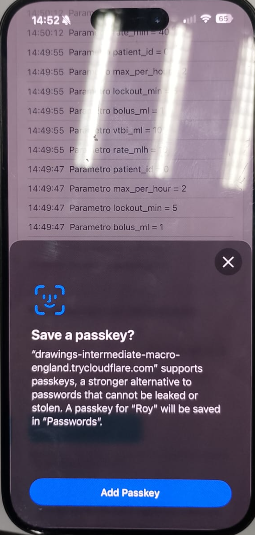
\includegraphics[width=\linewidth]{iphone_passkey_guardar.png}\caption{Registro: guardar la passkey}\end{subfigure}\hspace{1.2cm}
\begin{subfigure}{0.3\linewidth}\centering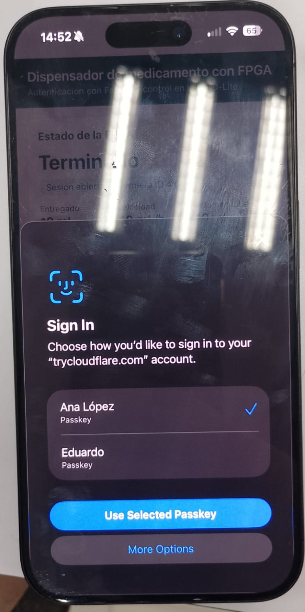
\includegraphics[width=\linewidth]{iphone_faceid_login.png}\caption{Inicio de sesión con Face ID}\end{subfigure}
\caption{Face ID en el iPhone sobre la página del dispensador servida por el túnel HTTPS.}
\label{fig:faceid}
\end{figure}

La Figura~\ref{fig:infusion} muestra la infusión en curso. Los LEDs de bomba y gota parpadean porque la bomba se enciende solo cuando faltan gotas, y el volumen entregado aumenta en el display. Con la enfermera fuera de sesión, la infusión continuó sin intervención de la laptop, ya que el programador y el lazo de control residen en la FPGA.

\begin{figure}[H]
\centering
\begin{subfigure}{0.32\linewidth}\centering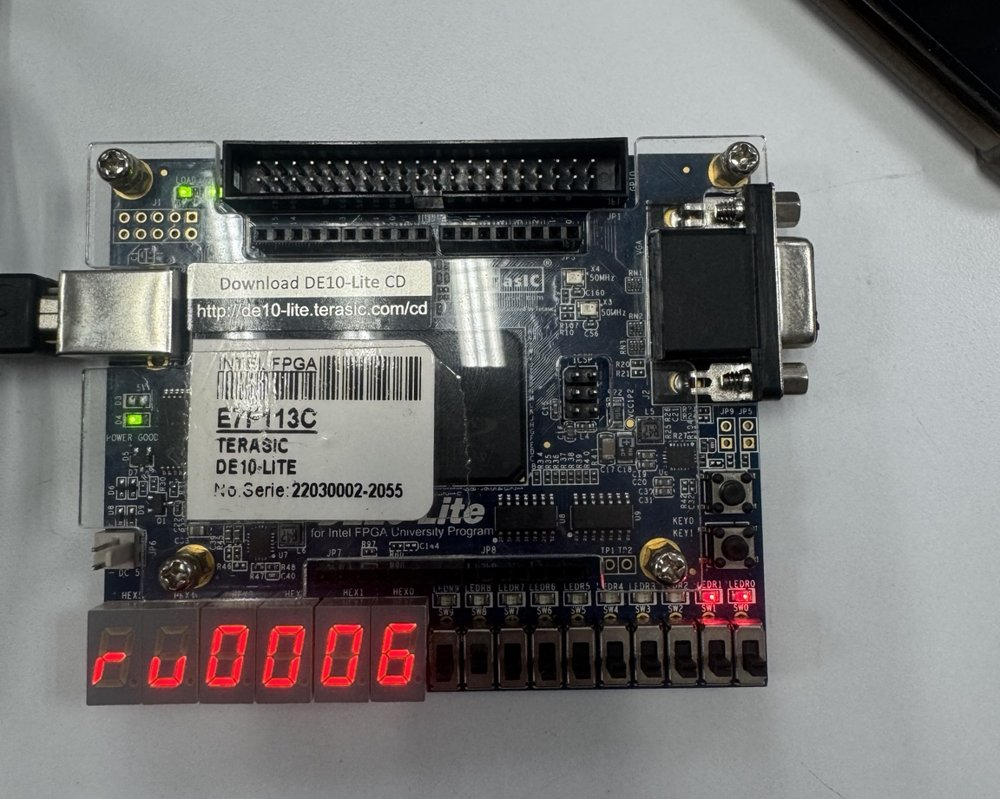
\includegraphics[width=\linewidth]{fpga_infusion_a.jpg}\caption{6~mL entregados}\end{subfigure}\hfill
\begin{subfigure}{0.32\linewidth}\centering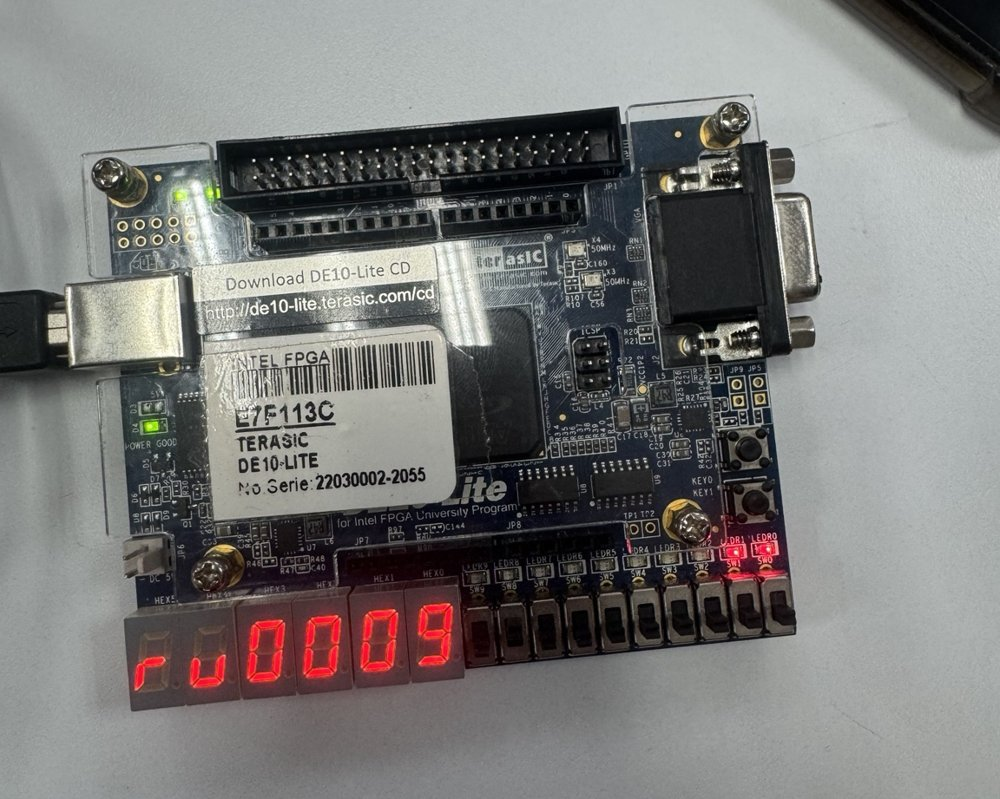
\includegraphics[width=\linewidth]{fpga_infusion_b.jpg}\caption{9~mL entregados}\end{subfigure}\hfill
\begin{subfigure}{0.32\linewidth}\centering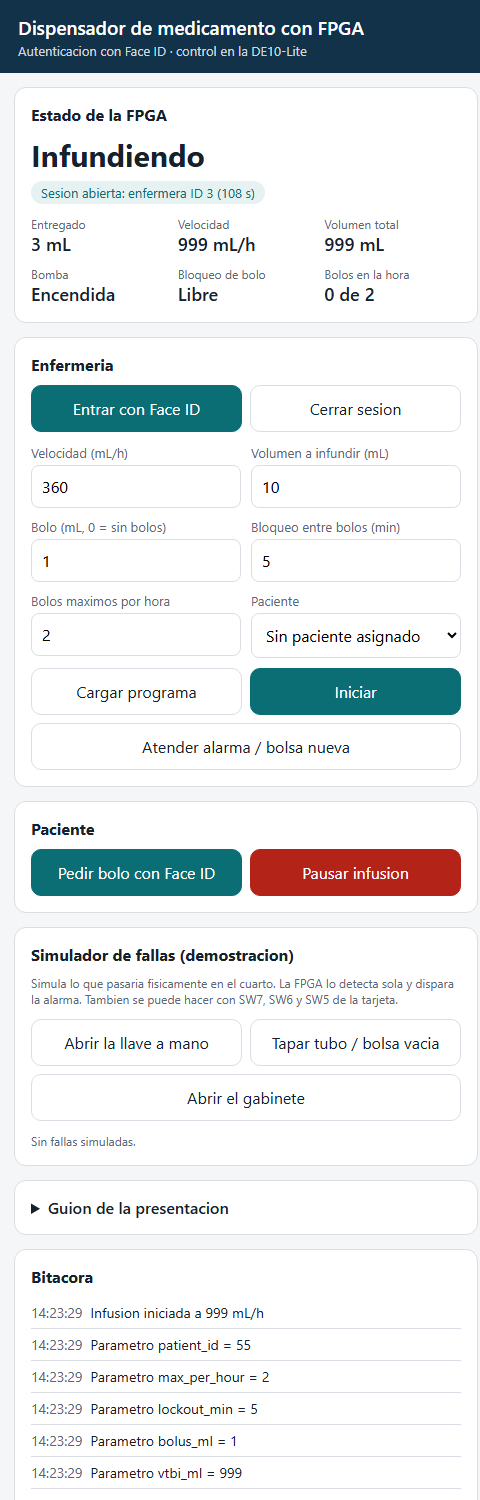
\includegraphics[width=\linewidth,trim=0 1170 0 0,clip]{web_infusion.png}\caption{Estado en la página}\end{subfigure}
\caption{Infusión en curso a 999~mL/h (\code{ru}).}
\label{fig:infusion}
\end{figure}

\subsection{Bolos y órdenes no autorizadas}
El paciente 55 obtuvo un bolo con su rostro y el segundo, pedido de inmediato, se negó por tiempo de bloqueo (Figura~\ref{fig:bolos}). Con SW1 activo, el display mostró los minutos de bloqueo restantes. Una solicitud con el rostro de otra persona se rechazó porque no correspondía al paciente asignado, y una velocidad de 0~mL/h se rechazó por estar fuera de rango. En simulación, con un máximo de 3 bolos por hora y 10~min de bloqueo, el cuarto bolo a los 30~min se negó por el límite horario y se concedió de nuevo a los 60~min, cuando el primero salió de la ventana.

\begin{figure}[H]
\centering
\begin{subfigure}{0.32\linewidth}\centering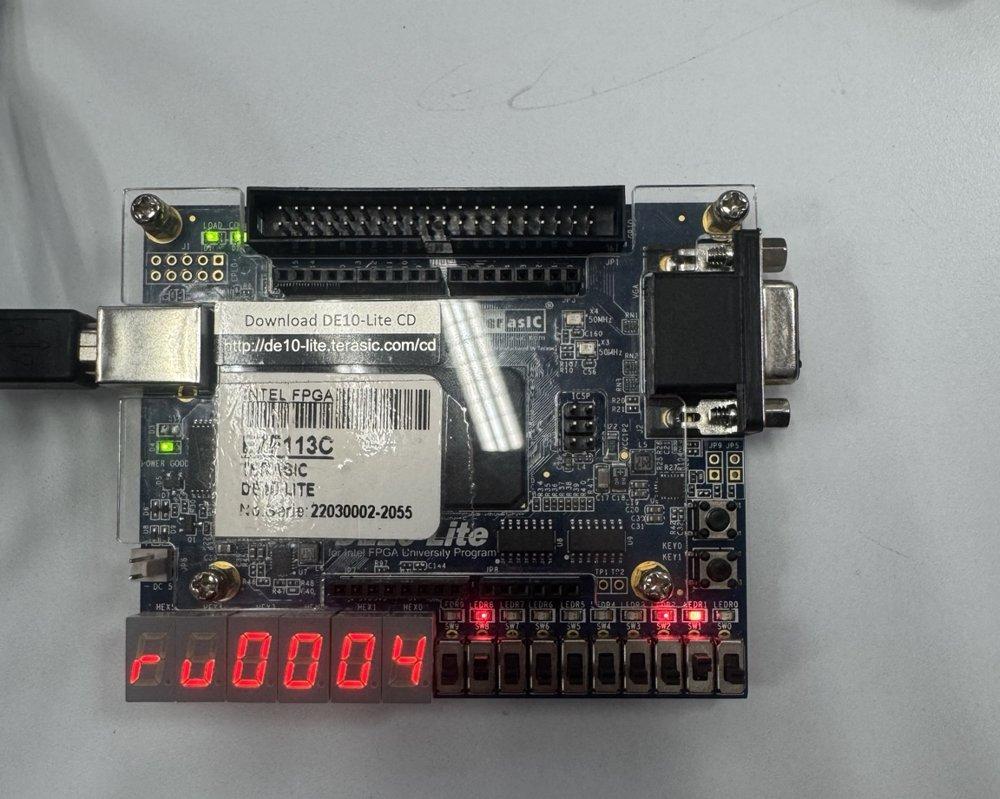
\includegraphics[width=\linewidth]{fpga_bloqueo.jpg}\caption{Bloqueo restante: 4~min}\end{subfigure}\hfill
\begin{subfigure}{0.32\linewidth}\centering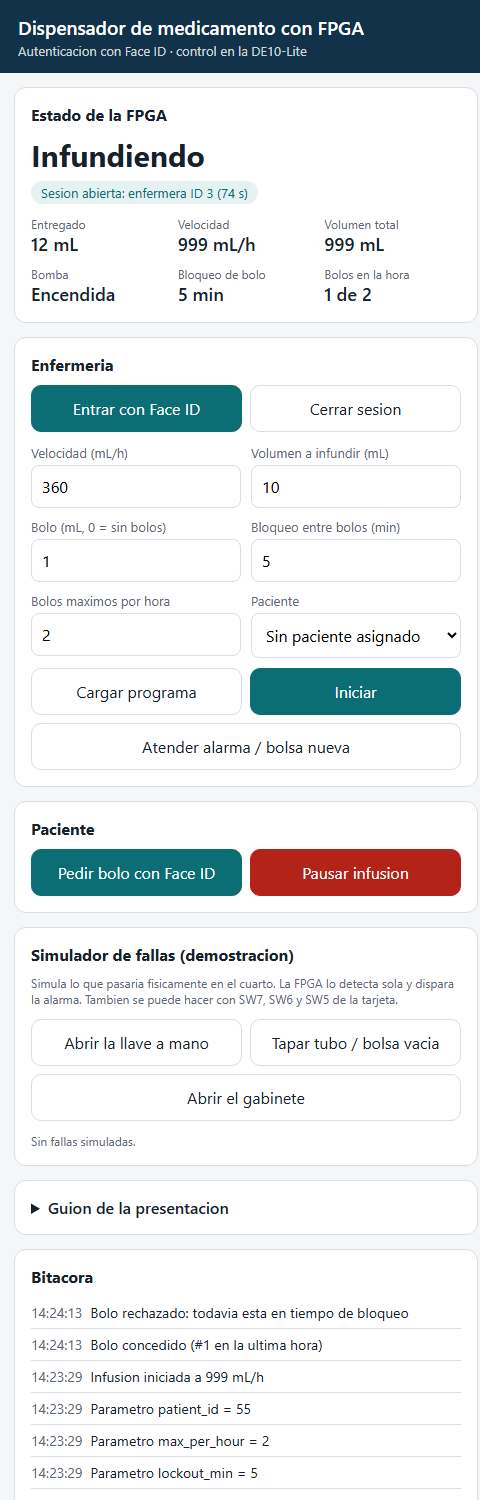
\includegraphics[width=\linewidth,trim=0 0 0 1230,clip]{web_bolos.png}\caption{Bolo concedido y negado}\end{subfigure}\hfill
\begin{subfigure}{0.32\linewidth}\centering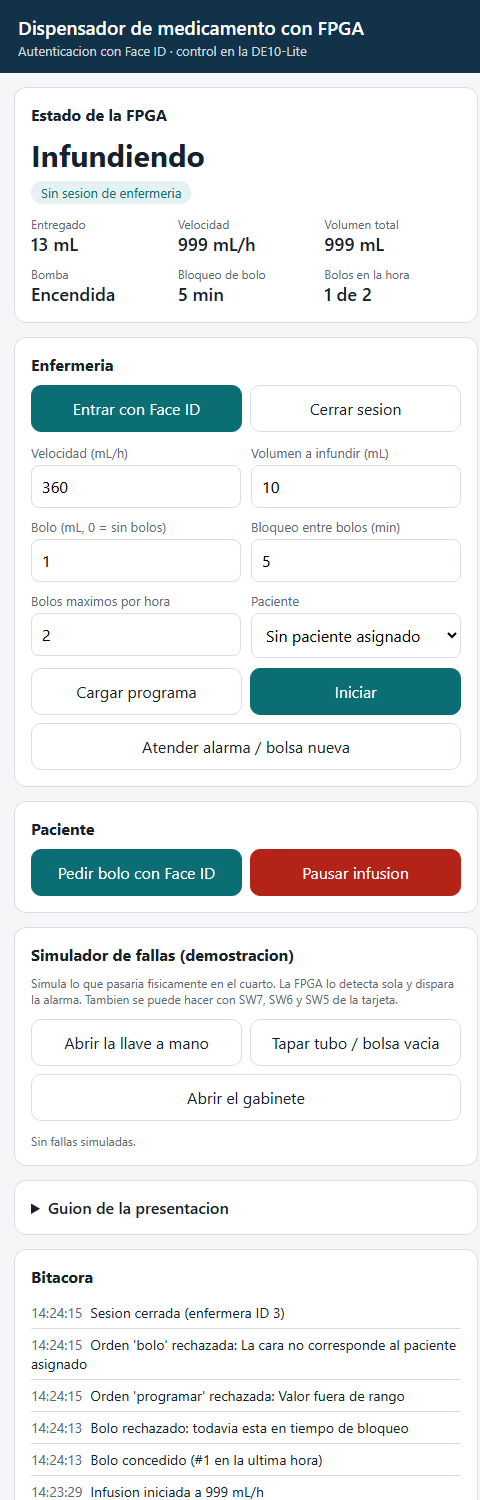
\includegraphics[width=\linewidth,trim=0 0 0 1230,clip]{web_rechazos.png}\caption{Órdenes rechazadas}\end{subfigure}
\caption{Limitador de bolos y rechazo de órdenes no autorizadas, registrados en la bitácora.}
\label{fig:bolos}
\end{figure}

Al pasar de la simulación a la tarjeta encontramos dos errores en el servidor que las pruebas automáticas no habían mostrado. Primero, enviamos 2000~mL/h desde la página y la FPGA recibió 976~mL/h. El campo de valor de la orden SET tiene 10 bits, así que el servidor cortaba el número ($2000 - 1024 = 976$) y la FPGA recibía un valor que sí estaba dentro de su rango, por lo que no tenía motivo para rechazarlo. Lo corregimos validando el rango en el servidor antes de empaquetar el valor; la FPGA conserva su propia validación de 1--999~mL/h. Segundo, pedimos un bolo durante el tiempo de bloqueo y el iPhone lo mostró como aceptado aunque la FPGA lo había negado. El servidor tomaba como respuesta el acuse de la orden, que llega antes de que el limitador decida. Ahora espera el evento de concesión o rechazo de la FPGA antes de responder al iPhone. Agregamos ambos casos a las pruebas del servidor. Con esto vimos que el acuse de que la FPGA recibió una orden no equivale al resultado de esa orden, y que la conversión entre los números del servidor y los campos de bits del hardware hay que probarla también con valores fuera de rango.

\subsection{Alarmas}
La Tabla~\ref{tab:tiempos} muestra los tiempos de detección medidos en la tarjeta desde la orden de simulación. La Figura~\ref{fig:alarmas} muestra las tres alarmas. En todos los casos la bomba se apagó, LEDR9 se encendió y la página mostró el aviso en rojo.

\begin{table}[H]
\centering
\caption{Tiempo de detección de cada falla en la tarjeta (999~mL/h).}
\label{tab:tiempos}
\begin{tabular}{lll}
\toprule
\textbf{Falla simulada} & \textbf{Alarma} & \textbf{Tiempo medido} \\
\midrule
Llave abierta a mano & Flujo libre & 0.7~s \\
Tubo tapado / bolsa vacía & Sin flujo & 5.6~s \\
Gabinete abierto sin sesión & Manipulación & 0.1~s \\
Gabinete abierto con sesión & Ninguna (permitido) & --- \\
\bottomrule
\end{tabular}
\end{table}

\begin{figure}[H]
\centering
\begin{subfigure}{0.32\linewidth}\centering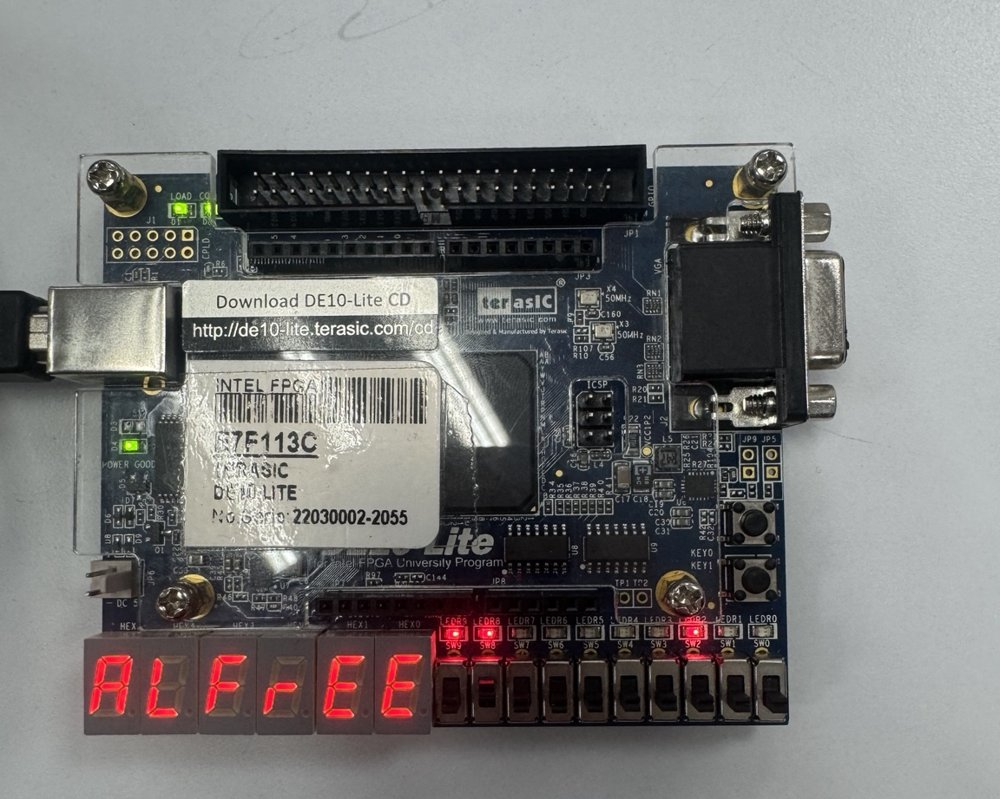
\includegraphics[width=\linewidth]{fpga_free.jpg}\caption{Flujo libre}\end{subfigure}\hfill
\begin{subfigure}{0.32\linewidth}\centering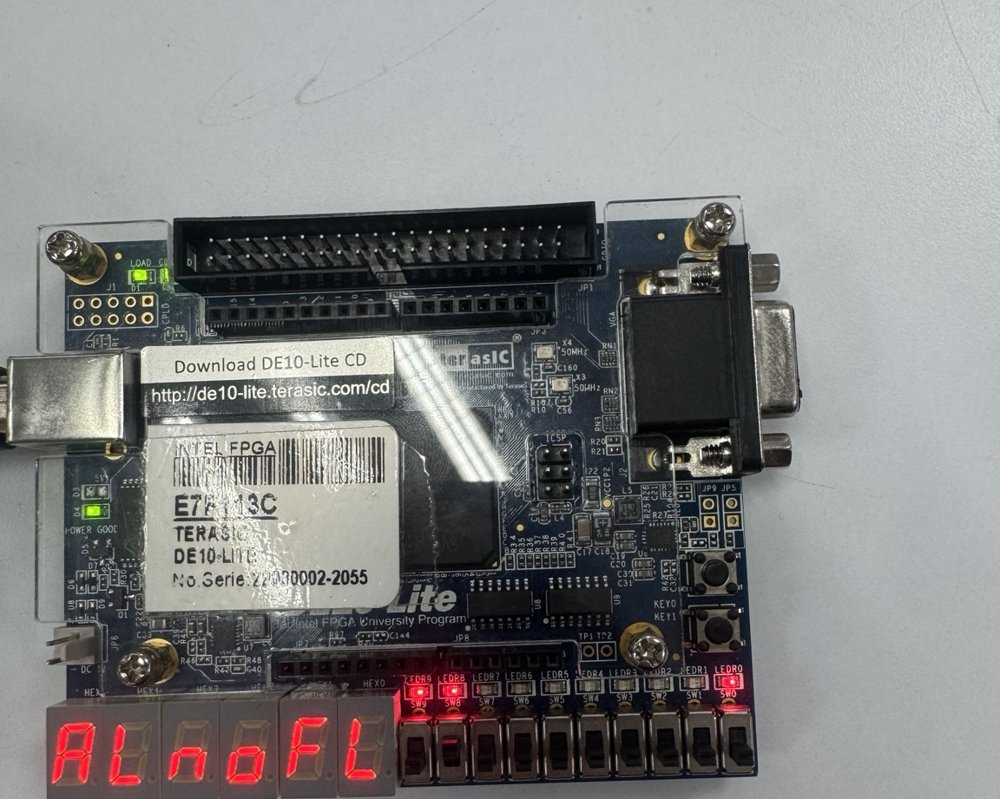
\includegraphics[width=\linewidth]{fpga_nofl.jpg}\caption{Sin flujo}\end{subfigure}\hfill
\begin{subfigure}{0.32\linewidth}\centering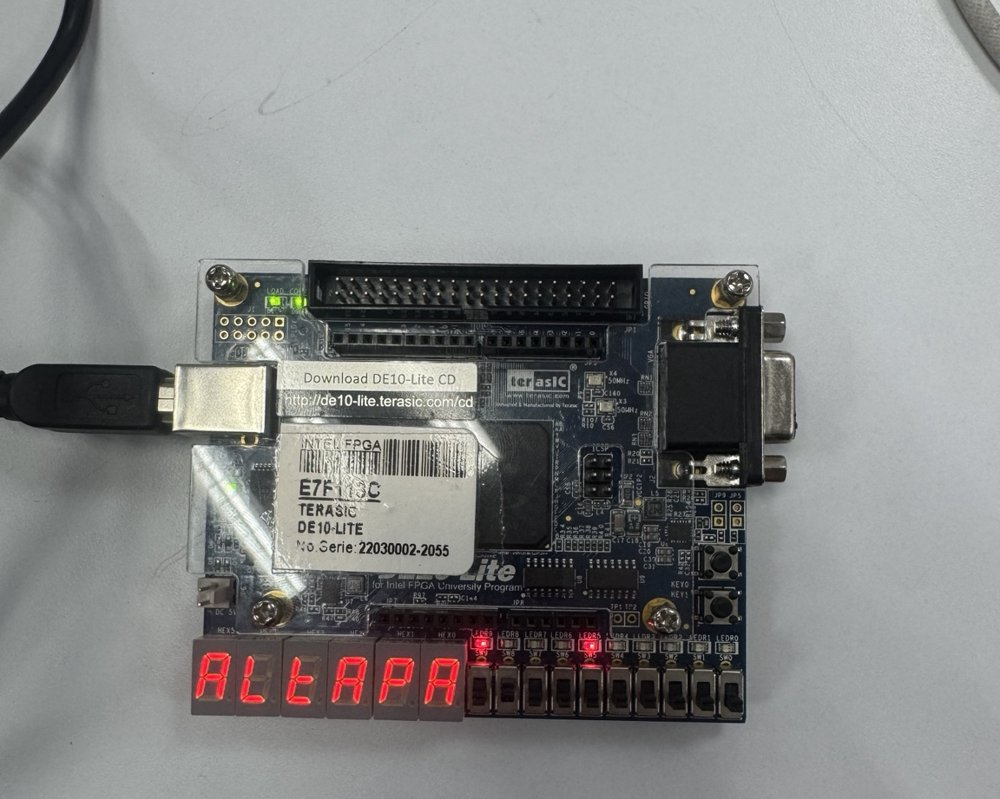
\includegraphics[width=\linewidth]{fpga_tapa.jpg}\caption{Manipulación}\end{subfigure}
\caption{Alarmas mostradas por la FPGA en los displays de siete segmentos.}
\label{fig:alarmas}
\end{figure}

El tiempo de 5.6~s para la ausencia de flujo se compone del umbral de 5~s más el tiempo hasta que la bomba se enciende por primera vez. En la primera versión, la fuga simulada producía una gota cada 400~ms, más lento que la bomba, y la alarma de flujo libre tardó 6.5~s; con una gota cada 120~ms, más cercano a un flujo sin control, bajó a 0.7~s. También se observó una alarma de sin flujo sin falla aparente: el volumen entregado era 0~mL, lo que indicaba que un interruptor había desconectado el modelo de goteo. Por eso se eliminó la opción de sensor externo en SW8 y se agregó el panel de simulación en la página, que deja la demostración menos expuesta a la posición de los interruptores.

La Figura~\ref{fig:cierre} muestra la alarma atendida por la enfermera y el fin de una infusión de 3~mL. Al llegar al volumen programado la bomba se detuvo sola, sin alarma.

\begin{figure}[H]
\centering
\begin{subfigure}{0.24\linewidth}\centering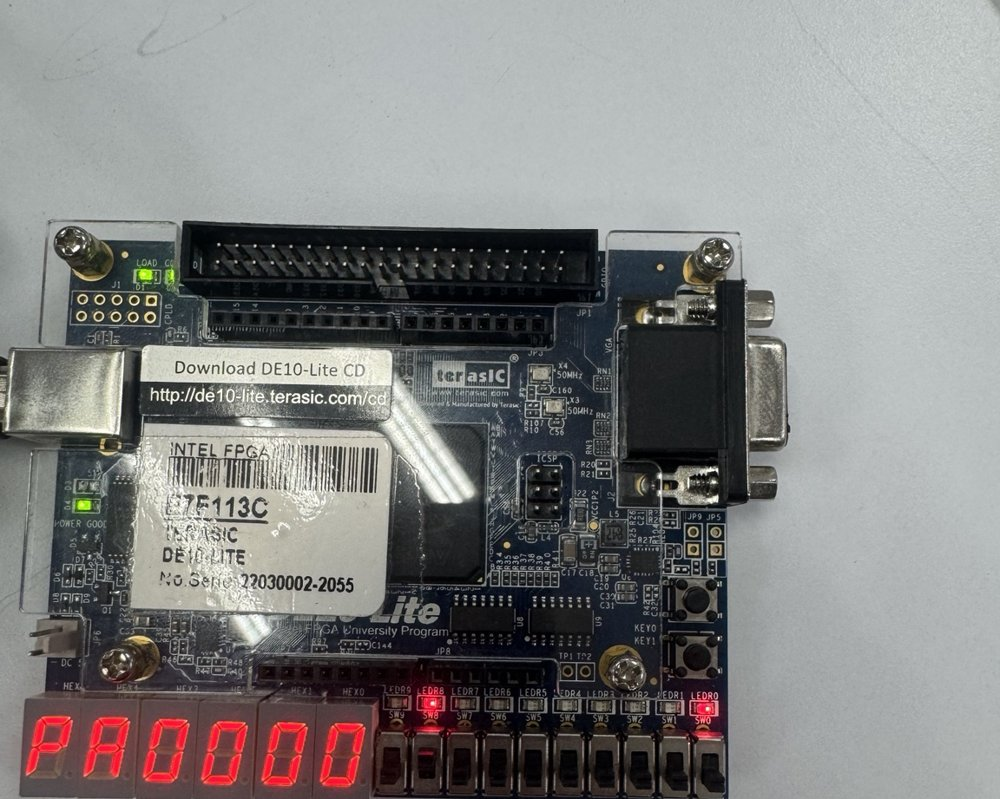
\includegraphics[width=\linewidth]{fpga_pausa.jpg}\caption{Alarma atendida}\end{subfigure}\hfill
\begin{subfigure}{0.24\linewidth}\centering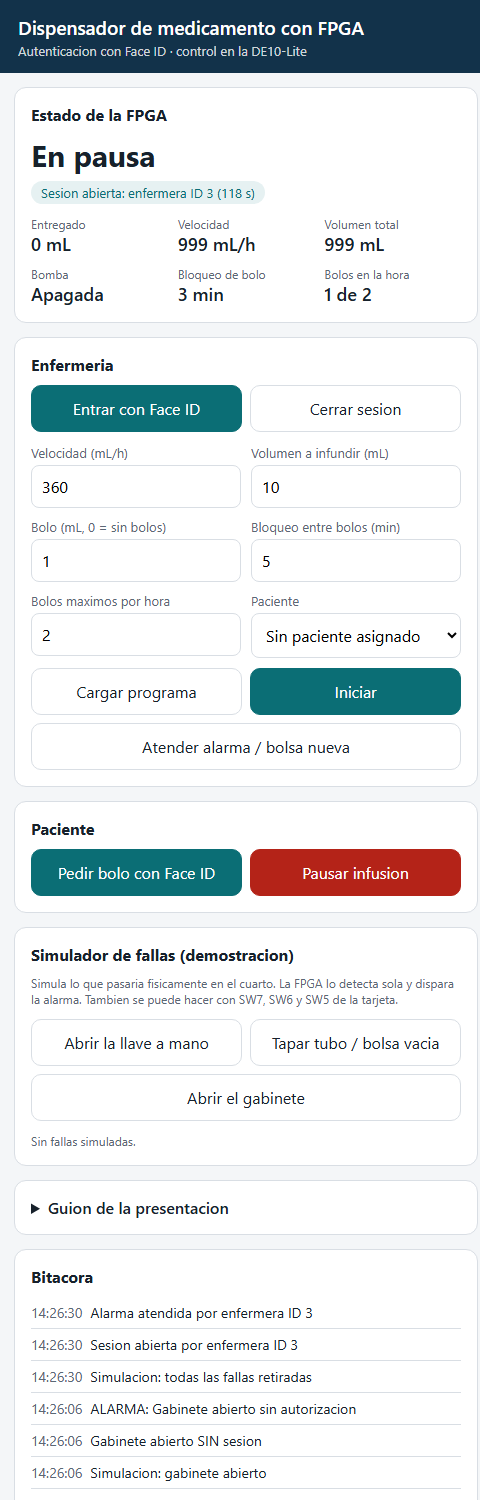
\includegraphics[width=\linewidth,trim=0 0 0 1230,clip]{web_atender.png}\caption{Bitácora}\end{subfigure}\hfill
\begin{subfigure}{0.24\linewidth}\centering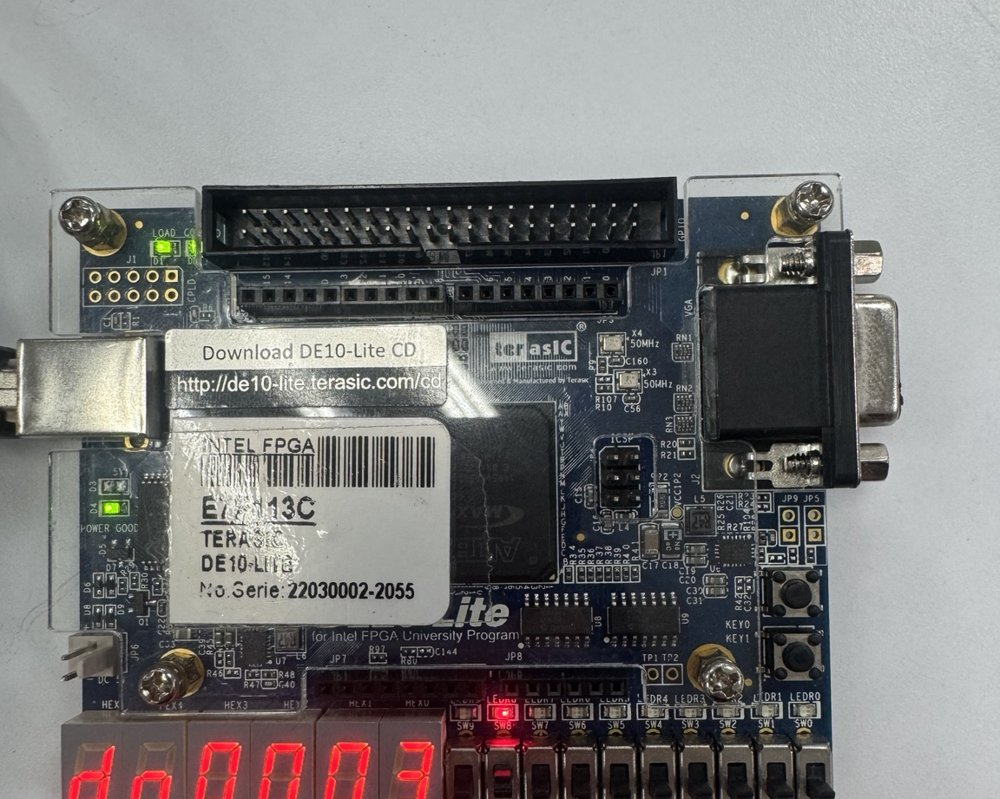
\includegraphics[width=\linewidth]{fpga_fin.jpg}\caption{Fin (\code{dn})}\end{subfigure}\hfill
\begin{subfigure}{0.24\linewidth}\centering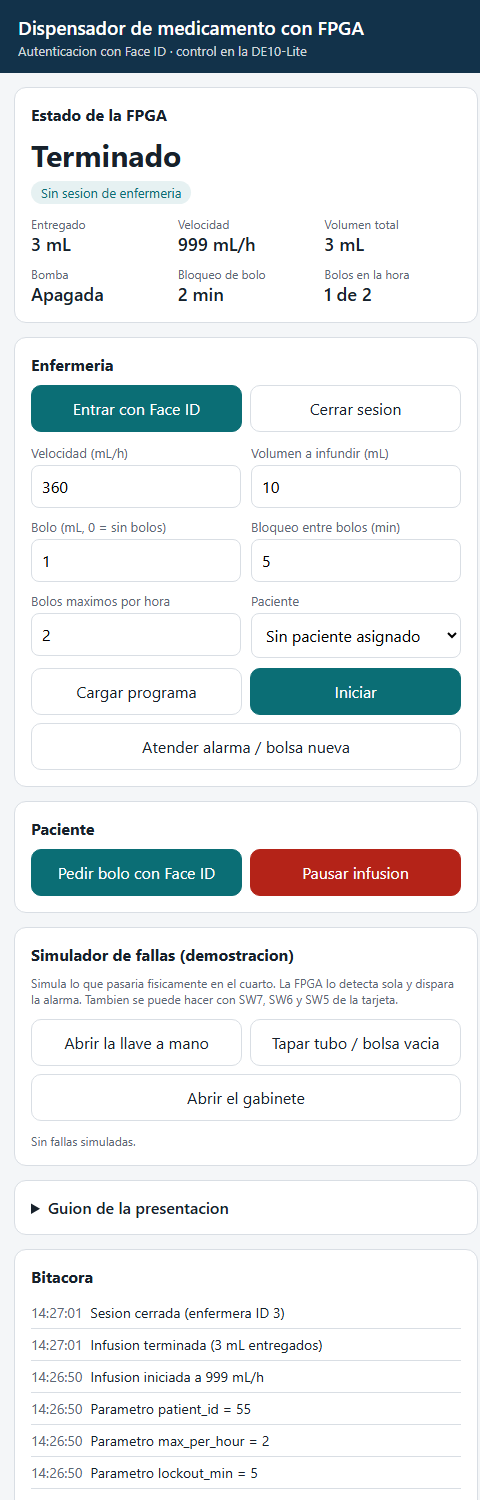
\includegraphics[width=\linewidth,trim=0 1170 0 0,clip]{web_fin.png}\caption{Página}\end{subfigure}
\caption{Atención de una alarma por la enfermera y fin de la infusión con 3~mL entregados.}
\label{fig:cierre}
\end{figure}

\subsection{Discusión}
La división de funciones planteada permitió cumplir con el objetivo de que la FPGA realizara la función principal del dispensador. La laptop se limitó a verificar la firma de Face ID y a transportar palabras de 32 bits, mientras que las decisiones sobre quién puede actuar, qué valores son válidos, cuándo se concede un bolo y cuándo debe detenerse la bomba se tomaron directamente en hardware. Esto quiere decir que, si la laptop llegara a enviar una orden indebida (por ejemplo, un bolo con un ID distinto al del paciente asignado o un parámetro fuera de rango), la FPGA la rechazaría y la dejaría registrada en la bitácora.

El uso del cable de programación como canal de datos evitó tener que agregar módulos de comunicación, aunque tiene como desventaja que la laptop debe permanecer conectada y con Quartus instalado. En un equipo real, el mismo protocolo de órdenes podría trasladarse a UART o Ethernet sin necesidad de modificar las reglas implementadas en la FPGA.

\subsection{Limitaciones}\label{sec:limitaciones}
La principal limitación del proyecto es que la bomba, la cámara de goteo y las fallas se simulan dentro de la FPGA, por lo que los resultados obtenidos demuestran la lógica de control y no el comportamiento hidráulico del equipo. De igual forma, la orden SIM existe únicamente para la demostración y no requiere autenticación, por lo que en un producto sería necesario eliminarla y leer sensores reales. Otro punto a considerar es que el servidor confía en la laptop para verificar las firmas; un atacante con control de la laptop podría abrir una sesión sin rostro, aunque seguiría limitado por los rangos y los límites de bolos de la FPGA. Por último, el túnel rápido cambia de dirección cada vez que se inicia, lo que obliga a registrar de nuevo los rostros, ya que cada passkey queda ligada a un dominio; para un uso continuo convendría contar con un dominio fijo.

% =============================================================== 4 CONCLUSIONES
\section{Conclusiones}\label{sec:conclusiones}
Se logró implementar de manera física sobre la tarjeta DE10-Lite un dispensador de medicamento líquido que únicamente acepta órdenes de personas autenticadas con Face ID. La FPGA controla la infusión gota a gota en lazo cerrado, limita los bolos del paciente y detecta tanto el flujo libre como la ausencia de flujo y la apertura no autorizada del gabinete, con tiempos de 0.7, 5.6 y 0.1~s respectivamente.

Las passkeys de WebAuthn permitieron aprovechar el Face ID del iPhone sin tener que desarrollar una aplicación ni comprar un sensor biométrico, mientras que el bloque In-System Sources and Probes hizo posible comunicar la laptop con la FPGA por el mismo cable de programación. En cuanto a recursos, el diseño ocupa el 5\,\% del dispositivo y cumple con los tiempos con margen.

Cabe destacar que las pruebas en la tarjeta revelaron errores que la simulación no había mostrado, como el truncamiento de un parámetro de 10 bits y la confirmación prematura de un bolo. Para una versión de uso clínico sería necesario conectar una bomba y un sensor de gotas reales, eliminar la simulación de fallas y llevar la verificación de identidad a un servidor dedicado con un dominio fijo.

% =============================================================== REFERENCIAS
\begin{thebibliography}{99}
\small
\bibitem{fda_pumps} U.S. Food and Drug Administration, ``Infusion pump improvement initiative,'' 2010. [Online]. Available: \url{https://www.fda.gov/medical-devices/infusion-pumps/infusion-pump-improvement-initiative}
\bibitem{webauthn} World Wide Web Consortium, \emph{Web Authentication: An API for Accessing Public Key Credentials, Level 2}, W3C Recommendation, Apr. 2021. [Online]. Available: \url{https://www.w3.org/TR/webauthn-2/}
\bibitem{apple_passkeys} Apple Inc., ``About the security of passkeys,'' Apple Support. [Online]. Available: \url{https://support.apple.com/en-us/102195}
\bibitem{apple_biometric} Apple Inc., ``Biometric security,'' in \emph{Apple Platform Security}. [Online]. Available: \url{https://support.apple.com/guide/security/biometric-security-sec067eb0c9e/web}
\bibitem{de10lite} Terasic Inc., ``DE10-Lite Development and Education Board.'' [Online]. Available: \url{https://www.terasic.com.tw/cgi-bin/page/archive.pl?Language=English&No=1021}
\bibitem{verilog} \emph{IEEE Standard Verilog Hardware Description Language}, IEEE Std 1364-2001, IEEE Standards Association. [Online]. Available: \url{https://standards.ieee.org/ieee/1364/2052/}
\bibitem{issp} Altera Corporation, ``Design debugging using In-System Sources and Probes,'' in \emph{Quartus Prime Standard Edition User Guide: Debug Tools}, ver. 18.1, cap. 8. [Online]. Available: \url{https://docs.altera.com/r/docs/683552/current}
\bibitem{jtag} \emph{IEEE Standard for Test Access Port and Boundary-Scan Architecture}, IEEE Std 1149.1-2013, IEEE Standards Association. [Online]. Available: \url{https://standards.ieee.org/ieee/1149.1/4484/}
\bibitem{chu} P. P. Chu, \emph{FPGA Prototyping by Verilog Examples}. Hoboken, NJ, USA: Wiley, 2008. [Online]. Available: \url{https://doi.org/10.1002/9780470374283}
\bibitem{flask} Pallets Projects, ``Flask documentation.'' [Online]. Available: \url{https://flask.palletsprojects.com/en/stable/}
\bibitem{pywebauthn} Duo Labs, ``py\_webauthn: Pythonic WebAuthn,'' GitHub repository. [Online]. Available: \url{https://github.com/duo-labs/py_webauthn}
\bibitem{cloudflare} Cloudflare Inc., ``Quick Tunnels,'' Cloudflare Tunnel documentation. [Online]. Available: \url{https://developers.cloudflare.com/tunnel/get-started/quick-tunnels/}
\bibitem{iverilog} S. Williams, ``Icarus Verilog.'' [Online]. Available: \url{https://steveicarus.github.io/iverilog/}
\end{thebibliography}

\end{document}
